\chapter{Background}
\label{ch:object-detection}
\section{Fundamentals of Object Detection}
% What's object detection? Describe the task itself, how it differs from  classification and other computer vision tasks. What are the usual approaches in the deep learning context (one-stage vs two-stage, anchor-based vs anchor-free, etc.)? What are the most common architectures and their characteristics? 
% highlight problems related to their structured outputs and the inherited challenges for gradient backpropagation 

Object detection is one of the fundamental task in computer vision that involves localizing and classifying multiple objects within an image. Unlike image classification and other tasks that assign a single label to an individual image, object detection requires predicting a set of bounding boxes, each associated with a class label and a confidence score. The challenging nature of this output stems from the variable cardinality of such sets, as the number of objects in an image can vary significantly, leading to complex structured prediction problems.

To address these challenges in a principled manner, it is useful to describe object detection as a structured prediction problem. This framework not only clarifies the task requirements but also provides a common language for comparing different detection architectures and loss functions.\\

Let an image be denoted as 
$
x \in \mathbb{R}^{H \times W \times C},
$
where $H$ and $W$ are the spatial dimensions and $C$ is the number of channels.
The output of an object detector is a finite set of detections:
$$
\mathcal{D} = \{ (b_i, y_i, s_i) \}_{i=1}^N,
$$
where:
\begin{itemize}
    \item $b_i = (x_i, y_i, w_i, h_i)$ represents the bounding box in pixel coordinates in COCO format (center position, width, height);
    \item $y_i \in \{1, \dots, K\}$ is the predicted class label, with $K$ the total number of object classes;
    \item $s_i \in [0,1]$ is the confidence score, often interpreted as the estimated probability that $b_i$ belongs to class $y_i$.
\end{itemize}

During training, ground-truth bounding boxes $b_i^\ast$ are typically transformed into target regression parameters relative to reference boxes (anchors or proposals) as:
$$
t_x = \frac{x^\ast - x_a}{w_a}, \quad
t_y = \frac{y^\ast - y_a}{h_a}, \quad
t_w = \log \frac{w^\ast}{w_a}, \quad
t_h = \log \frac{h^\ast}{h_a},
$$
where $(x_a, y_a, w_a, h_a)$ are the anchor box parameters, and $(x^\ast, y^\ast, w^\ast, h^\ast)$ are the corresponding ground-truth parameters.

The specific optimization objectives used for bounding box regression and classification are detailed in Section~\ref{sec:loss_functions}, following the description of the detection architectures.

The object detection task can thus be formalized as learning a function:
$$
f_\theta: \mathbb{R}^{H \times W \times C} \to \mathcal{P}(\mathbb{R}^4 \times \{1, \dots, K\} \times [0,1]),
$$
parameterized by $\theta$, that maps an input image to a set of bounding box--label--score triples.
The set-valued nature of $\mathcal{P}(\cdot)$ reflects that the number of detections varies between images.

This formalization underpins the taxonomy of detection architectures discussed in the following section, where we distinguish between one-stage and two-stage approaches, anchor-based and anchor-free formulations, and their respective training and inference paradigms.

\subsubsection{Feature Pyramid Networks (FPN)}
Before diving into the specific architectures, we introduce a widely used component in most object detection models: the Feature Pyramid Network (FPN).

Objects appear at widely varying scales, early CNN backbone layers produce high-resolution but semantically weak features (shallow layers), while deeper layers produce low-resolution but semantically strong features.
FPNs fuse these to obtain semantically strong, multi-scale feature maps at multiple resolutions, enabling detectors to handle small and large objects efficiently with a single backbone pass (as opposed to costly image pyramids)~\cite{lin2017fpn}.\\

Let $\{C_2,C_3,C_4,C_5\}$ be backbone feature maps with strides $\{4,8,16,32\}$ w.r.t.\ the input.
FPN builds $\{P_2,P_3,P_4,P_5\}$ by a top–down pathway and lateral merges as shown in Figure~\ref{fig:fpn-lateral}.

\begin{figure}[h]
    \centering
    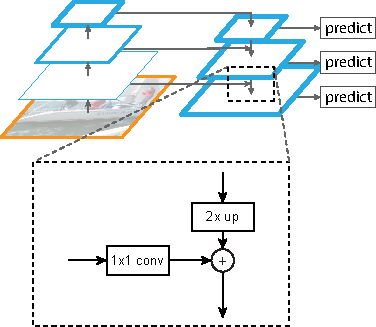
\includegraphics[]{images/fpn-lateral.pdf}
    \caption{A building block illustrating the lateral connection and
    the top-down pathway, merged by addition \cite{lin2017fpn}}
    \label{fig:fpn-lateral}
\end{figure}


\subsection{One-Stage vs Two-Stage Detectors}

Object detectors can be broadly categorized into \emph{one-stage} and \emph{two-stage} paradigms. Both ultimately predict a variable-sized set of detections $\mathcal{D} = \{(b_i, y_i, s_i)\}$, but they differ in how they structure intermediate computations and where they allocate capacity for localization vs.\ classification.

\subsubsection{Two-stage detectors.}
Two-stage methods decompose detection into proposal generation followed by proposal classification and box refinement. Let $g_{\phi}$ denote a proposal mechanism (e.g., a region proposal network operating on a shared backbone), which maps an image $x$ to a set of candidate regions $\mathcal{P}$:
$$
\mathcal{P} = g_{\phi}(x) = \{p_j\}_{j=1}^{M}.
$$
A second function $f_{\theta}$ then classifies and refines these regions to produce final detections:
$$
\mathcal{D} = f_{\theta}(x, \mathcal{P}).
$$
Operationally, the pipeline is:
\begin{enumerate}
    \item Backbone (optionally with a feature pyramid) extracts multi-scale features from $x$.
    \item A proposal generator produces a sparse set of regions $\mathcal{P}$ (typically with non-maximum suppression to reduce redundancy).
    \item Per-region features are pooled/aligned from the shared feature maps and passed to a detection head to output class scores and refined boxes.
\end{enumerate}

The idea underlying two-stage detectors is to incentivise accuracy by first generating a manageable number of promising candidates, which can then be processed and refined with more complex per-region heads. This also allows for a more efficient use of computational resources, as the second stage can focus on a smaller set of regions rather than processing the entire image densely.
But unfortunately, this approach introduces a fair amount of complexity requiring careful design.

\subsubsection{One-stage detectors.}
One-stage methods simplify the detection pipeline by predicting detections directly from the shared feature maps without an explicit proposal stage. This design is motivated by the desire to maximize throughput and reduce latency, particularly in real-time applications. This type of detection is often referred to as \emph{dense predictions} because it involves predicting detections at every spatial location of the feature maps, often having to take into account hundreds of thousands of locations per image.
Conceptually, it implements a direct mapping
$$
\mathcal{D} = h_{\psi}(x),
$$
where $h_{\psi}$ produces, for each spatial location (and possibly for multiple predefined reference shapes), joint classification scores and box parameters. The pipeline is:
\begin{enumerate}
    \item Backbone (optionally with a feature pyramid) extracts multi-scale features from $x$.
    \item Lightweight prediction heads applied densely over feature maps output $(b, y, s)$ candidates.
    \item A single-stage post-processing (e.g., top-$k$ filtering and non-maximum suppression) yields $\mathcal{D}$.
\end{enumerate}
This design maximizes throughput and simplifies the graph, but operates under severe class imbalance, due to the fact that most locations tend to be related to a generic background class, and thus the model has to learn to distinguish between a very large number of background locations and a comparatively small number of foreground locations. This imbalance is often addressed with specialized loss functions, such as the Focal Loss \cite{lin2018focalloss}, which down-weights easy-to-classify examples and focuses training on hard negatives.
The precision of the predictions often relies on effective assignment and post-processing techniques.
An alternative way of addressing this imbalance, ironically, is to use a two-stage approach, where the first stage takes care of separating the foreground (potential candidates) from the background.

\paragraph{Comparative characteristics.}
One might ask "Which paradigm is better then?" and the answer would be, as usual, "it depends". One-stage detectors are generally faster and more resource-efficient, and that is because they were intended to address the latency and throughput requirements of real-time applications. This comes at the cost of some accuracy that two-stage detectors can achieve with their more careful filtering mechanisms and (usually) more complex per-region heads that come at the cost of increased compatuational requirements and latency. And similarly one-stage detectors, they were designed to be accurate rather than fast.

Ideally one would like to have the best of both worlds, and we can find in literature a number of approaches that tries to reach two-stage performance with one-stage efficiency, such as the RetinaNet and YOLO \cite{lin2018focalloss,redmon2016yolo}.

We can summarize the main differences between one-stage and two-stage detectors as follows:
\begin{itemize}
    \item \textbf{Computation.} Two-stage: cost scales with the number of proposals $M$ (feature pooling and per-RoI head). One-stage: cost scales with the number of feature locations (and reference shapes) processed densely.
    \item \textbf{Capacity allocation.} Two-stage allocates more parameters per candidate via the second-stage head; one-stage relies on shallow, shared heads and benefits from strong multi-scale features.
    \item \textbf{Class imbalance.} One-stage training observes extreme foreground/background imbalance due to dense supervision; two-stage partially mitigates this by filtering with proposals and sampling strategies.
    \item \textbf{Latency/throughput.} One-stage typically achieves lower latency and higher FPS; two-stage often offers higher accuracy at increased computational cost.
    \item \textbf{Post-processing.} Two-stage commonly applies suppression both after proposal generation and after final classification; one-stage applies it once on dense predictions (often per class).
\end{itemize}


% \paragraph{Outlook.}
% In what follows, we instantiate these paradigms with canonical representatives: a one-stage detector with dense predictions, and a two-stage detector with proposals followed by RoI-level classification and refinement, both using feature pyramids to extract multi-scale features. We subsequently discuss anchor-based vs.\ anchor-free formulations, which apply orthogonally to both paradigms.


\subsection{Anchor-Based vs.\ Anchor-Free}

Object detectors differ not only by staging (one- vs.\ two-stage) but also by how they parameterize candidate boxes. The two prevailing choices are \emph{anchor-based} (predefined reference boxes) and \emph{anchor-free} (direct box prediction without references). This design is largely orthogonal to the staging paradigm.

\subsubsection{Anchor-based detectors}
\label{sec:anchor_based_detectors}
Let $\mathcal{A}=\{a_k\}_{k=1}^{K}$ be a set of predefined anchors tiled over feature maps. 
Each anchor $a_k=(x_a,y_a,w_a,h_a)$ serves as a reference against which a detector predicts offsets $(t_x,t_y,t_w,t_h)$ to obtain a box:
$$
x = x_a + w_a t_x \quad
y = y_a + h_a t_y \quad
w = w_a e^{t_w} \quad
h = h_a e^{t_h}
$$

Anchors are generated at multiple scales and aspect ratios per spatial location and per FPN level $\ell$ (with stride $s_\ell$), e.g.\ scales $\{s_\ell \cdot \alpha\}$ and ratios $r \in \{1\!:\!2,\,1\!:\!1,\,2\!:\!1\}$.
The number of anchors generated for each image tends to be large, but since we're considering the spatial locations of the feature maps, and not the original image, this number is still manageable, although it can still be in the order of hundreds of thousands, depending on the number of feature maps, stride, number of scales, aspect ratios and size of the image.\\

Training uses \emph{IoU-based assignment}: for ground-truth boxes $\{b_i^\ast\}$, compute $M_{ik}=\mathrm{IoU}(b_i^\ast,a_k)$; for some given $\tau_{\text{pos}}, \tau_{\text{neg}} \in [0, 1]$ mark $a_k$ positive if $M_{ik}\ge \tau_{\text{pos}}$ for some $i$, negative if $M_{ik}\le \tau_{\text{neg}}$, and ignore otherwise. 

We now have the anchors partitioned into $\mathcal{A}^+$ (positive), $\mathcal{A}^-$ (negative), and $\mathcal{A}^0$ (ignored).
Positives receive a foreground class label $y^\ast$ and regression targets $t_k$; negatives receive the background label; ignored anchors are excluded from loss computation.
Training thus optimizes
$$
\mathcal{L}
= \frac{1}{N_{\text{cls}}}\sum_{k \in \mathcal{A}^+ \cup \mathcal{A}^-} \ell_{\text{cls}}(\hat{c}_k, c_k)
\;+\;
\lambda\,\frac{1}{N_{\text{reg}}}\sum_{k \in \mathcal{A}^+} \ell_{\text{reg}}(\hat{t}_k, t_k),
$$
where $\ell_{\text{cls}}$ is the classification/objectness loss and $\ell_{\text{reg}}$ (e.g., Smooth-$L_1$ or IoU-based) is applied \emph{only} to positives.
Negatives contribute \emph{only} to classification as background; ignored anchors contribute to neither term.

\paragraph{Suppressing redundancy.}
As seen in this section, anchor-based detectors generate a large number of anchors, many of which are near-duplicates (they overlap with the same ground-truth boxes). Ideally we would like only one anchor, hence one detection, per ground-truth, therefore we need a post-processing procedure to remove these redundant detections.

This is typically done in two steps: we first keep the top-$k$ detections per level/class, where $k$ is an hyperparameter (pre-NMS step), and then we apply Non-Maximum Suppression (NMS) to remove overlaps, producing the final set $\mathcal{D}$ \cite{neubeck2006efficient}.
Given a set of competing detections $\mathcal{D} = \{(b_i, y_i, s_i)\}$, NMS iteratively selects the detection with the highest score $s_i$ and removes all other detections that overlap with it above a threshold $\tau_{\text{nms}}$ (typically $0.5$). The process continues until no detections remain above the threshold.
As a result, NMS produces a final set of detections $\mathcal{D} = \{(b_i, y_i, s_i)\}$ that are non-overlapping and have the highest scores among the competing detections.
This procedure is clearly non-differentiable, and thus it is not possible to backpropagate through it, hence we always backpropagate on the pre-NMS detections.


\subsubsection{Anchor-free detectors.}
Anchor-free methods remove the predefined anchor set $\mathcal{A}$: each feature-map location $p$ is supervised directly.
A common approach is the one used in FCOS, which assigns each location $p=(x_p, y_p)$ to at most one ground-truth box $b^\ast$ if $p \in b^\ast$ (optionally restricted to a center region and a size range matched to level $\ell$).
After assignment, the location $p$ is labeled positive with class $y^\ast$ and regression targets given by distances to the four sides of $b^\ast$:
$$
\ell_p = x_p - x^\ast_{\text{left}},\quad
t_p = y_p - y^\ast_{\text{top}},\quad
r_p = x^\ast_{\text{right}} - x_p,\quad
b_p = y^\ast_{\text{bottom}} - y_p,
$$
decoded at inference as $[x_p-\ell_p,\; y_p-t_p,\; x_p+r_p,\; y_p+b_p]$.
Locations not assigned to any box act as background in the classification loss and do not contribute to regression.
Many designs also predict a per-location quality term (e.g.\ ``centerness'') to down-weight ambiguous border locations. 
Alternative anchor-free formulations include keypoint-based representations (e.g.\ object centers or corners) with local offsets~\cite{tian2019fcos,law2019cornernet,duan2019centernet}.\\

Anchor-free models avoid anchor tuning and can better handle unusual aspect ratios, but rely on effective assignment rules (inside-box, center sampling, size ranges) and robust post-processing.

\paragraph{Comparison and practical notes.}
\begin{itemize}
    \item \textbf{Design knobs} Anchor-based: choose scales/ratios, IoU thresholds, per-level priors. Anchor-free: choose assignment region, size ranges per level, and optional quality terms.
    \item \textbf{Label assignment} Anchor-based uses $\mathrm{IoU}$ with thresholds; anchor-free uses geometric inclusion at locations (often with center sampling). Advanced heuristics (e.g., ATSS/OTA) can be applied to either family \cite{zhang2020atss,ge2021ota}.
    \item \textbf{Computational profile} Similar dense heads; anchor-free can reduce memory and labels by removing large anchor sets.
\end{itemize}



\section{RetinaNet}
% a one-stage anchor-based architecture, essentially a toned-down Faster R-CNN, this is why i'd describe it first
% Describe the its architecture and components, address that it is born to address the class imbalance problem with the Focal Loss introduction, and its intended for medical imaging applications


RetinaNet is a one-stage, anchor-based detector that combines a backbone with a feature pyramid and two lightweight, densely-applied heads (classification and regression). Its key contribution is the \emph{focal loss}, which mitigates extreme foreground/background imbalance in dense prediction~\cite{lin2018focalloss}.

\begin{figure}[h]
    \centering
    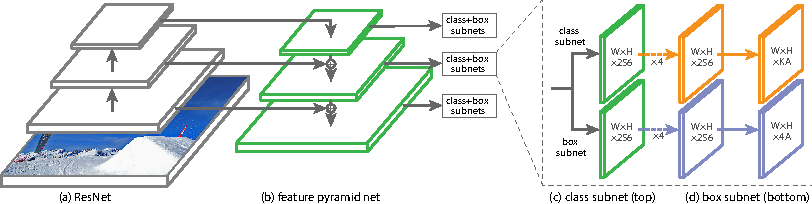
\includegraphics[page=1,width=\linewidth]{images/retinanet.pdf}
    \caption{RetinaNet architecture overview \cite{lin2018focalloss}}
    \label{fig:retinanet}
\end{figure}


\subsubsection{Architecture}
A convolutional backbone (e.g., ResNet) feeds a feature pyramid $\{P_\ell\}$ (typically $P_3$--$P_7$). 
At each pyramid level $\ell$ with spatial size $H_\ell \times W_\ell$, and stride $s_\ell$, a set of $A$ anchors per location is tiled. 
Two subnetworks are applied at each level of the pyramid, producing per-anchor outputs:
\begin{itemize}
    \item \emph{Classification head:} a small CNN produces per-class logits $\hat{z}_{\ell,ij,a,c}$, using independent sigmoids (no softmax) over $c \in \{1,\dots,K\}$.
    \item \emph{Regression head:} a parallel CNN predicts box deltas $\hat{t}_{\ell,ij,a}=(\hat{t}_x,\hat{t}_y,\hat{t}_w,\hat{t}_h)$.
\end{itemize}

Once we obtain the structured outputs from the network, we apply the post-processing steps discussed 
in Section~\ref{sec:anchor_based_detectors} to discard redundant detections.

\paragraph{Focal Loss.}

As previously mentioned, RetinaNet introduced the \emph{focal loss} to address the extreme class imbalance in dense predictions.
It essentially down-weights easy to classify examples and focuses training on hard negatives (Figure~\ref{fig:focal-loss}), which is particularly useful in medical imaging where the background class can dominate the training set. To do so it adds a modulating factor $(1-p_t)^\gamma$ to the cross-entropy loss, with a focus parameter $\gamma$. The focal loss is hence defined as follows:

$$
\mathrm{FL}(p_t) = -\,\alpha\,(1-p_t)^{\gamma}\,\log(p_t),
$$
with typical $\alpha{=}0.25$, $\gamma{=}2$.\\
\begin{figure}[h]
    \centering
    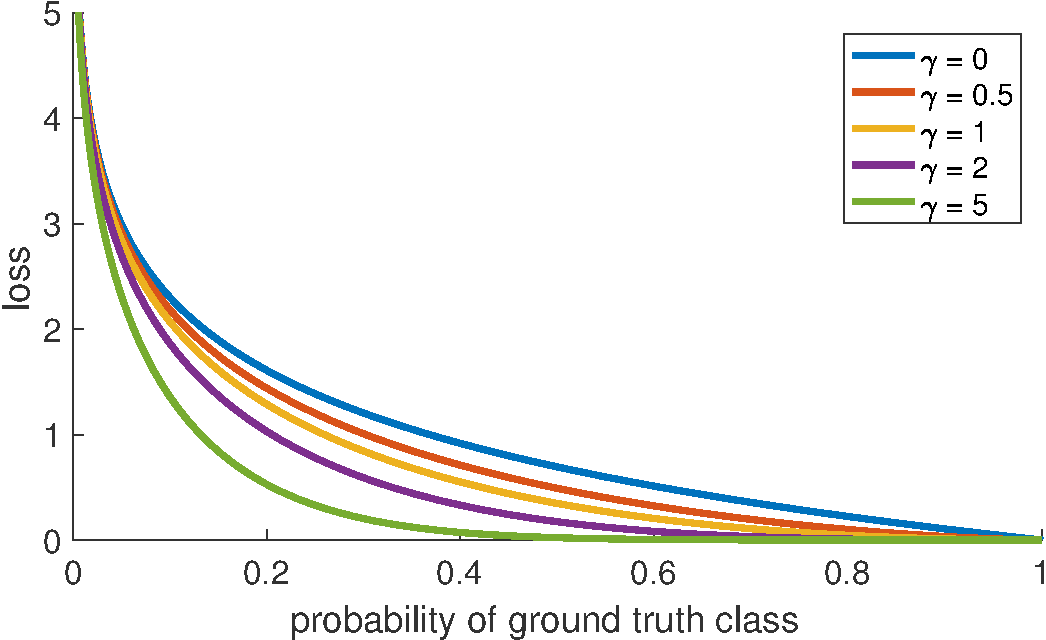
\includegraphics[width=0.55\linewidth]{images/focal-loss.pdf}
    \caption{Focal loss at different $\gamma$ values \cite{lin2018focalloss}. When $\gamma=0$, it is equivalent to cross-entropy loss. As $\gamma$ increases, the loss focuses more on hard examples, down-weighting easy ones.}
    \label{fig:focal-loss}
\end{figure}


\section{Faster R-CNN}
% two-stage anchor-based architecture, the most common one and the one that is used in most of the literature.
% Describe its components, RPN, RoI pooling etc., it is the culmination of the R-CNN family of architecutres.
% f

Faster R-CNN is a two-stage, anchor-based detector that couples a Region Proposal Network (RPN) with a per-region classifier and regressor~\cite{ren2016fasterrcnn}. A shared backbone (we consider one using FPN) feeds both stages.

\begin{figure}[h]
    \centering
    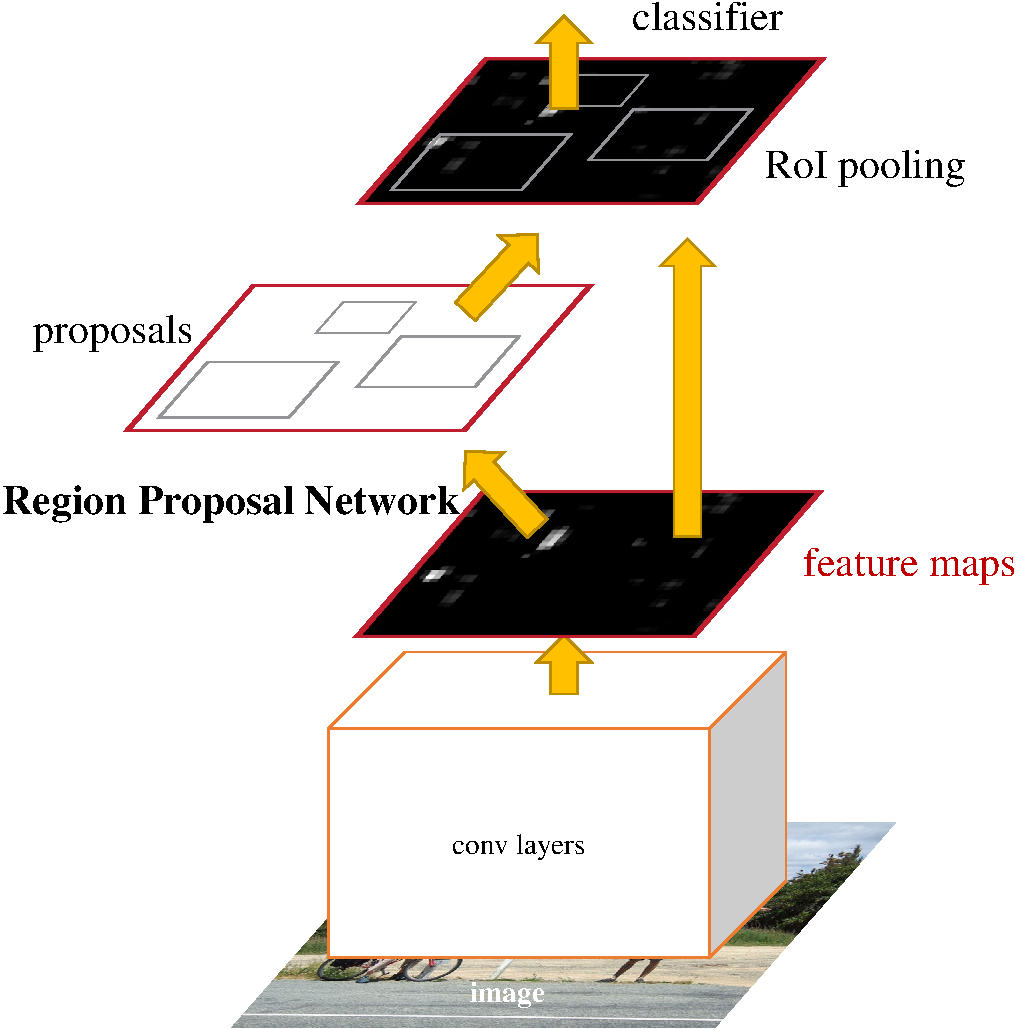
\includegraphics[width=0.6\linewidth]{images/fasterrcnn.pdf}
    \caption{Faster RCNN architecture overview \cite{ren2016fasterrcnn}}
    \label{fig:fasterrcnn}
\end{figure}


\subsubsection{Region Proposal Network (RPN).}
At each feature-map location and for $A$ anchors $a_k=(x_a,y_a,w_a,h_a)$, the RPN predicts:
\begin{itemize}
    \item objectness logits $\hat{o}_k$ (binary);
    \item box deltas $\hat{t}_k=(\hat{t}_x,\hat{t}_y,\hat{t}_w,\hat{t}_h)$.
\end{itemize}
At this stage we do not have any class information, but rather we unify all classes into a single \emph{object} against a \emph{background} class, hence the binary classification. We call \emph{objectness} the probability that an anchor contains an object, regardless of its initial class. Such probability is typically obtained by applying a sigmoid activation to the logits $\hat{o}_k$.\\
Anchors are assigned to ground-truth boxes by IoU thresholds: positives $\mathcal{A}^+$, negatives $\mathcal{A}^-$, ignored $\mathcal{A}^0$. Positives receive class $1$ and regression targets $t_k$ (standard parameterization),
$$
t_x=\frac{x^\ast-x_a}{w_a},\quad
t_y=\frac{y^\ast-y_a}{h_a},\quad
t_w=\log\frac{w^\ast}{w_a},\quad
t_h=\log\frac{h^\ast}{h_a}.
$$

At the end of the RPN, we filter the proposals by objectness score $\hat{o}_k$ and apply non-maximum suppression (NMS) to obtain a sparse set of proposals $\mathcal{P}$, which are then passed to the second stage.\\

We notice how the RPN is a fully convolutional network, therefore the size of input has not to be fixed, although it will increase the number of anchors and thus the computational cost.

\paragraph{Second-stage head.}
The second stage process starts with RoIAlign, a procedure that pools features from the shared backbone for each proposal into a fixed-size tensor $F_j$ (e.g., $7{\times}7{\times}C$) without quantization errors \cite{he2018maskrcnn}. This is done by bilinear interpolation of the feature maps at the proposal locations, which avoids the quantization issues that arise with max pooling, that was a common issue in the original R-CNN architectures using RoIPooling instead.

A per-RoI head predicts:
\begin{itemize}
    \item class logits $\hat{z}_{j,c}$ for $c\in\{1,\dots,K\}$ (softmax over $K{+}1$ including background);
    \item refined box deltas $\hat{u}_{j,c}$ (class-specific) or $\hat{u}_j$ (class-agnostic).
\end{itemize}
With labels $(y_j^\ast, u_j^\ast)$ from matching $p_j$ to ground truth, the loss is
$$
\mathcal{L}_{\text{RoI}}
=\frac{1}{N_{\text{roi}}}\sum_{j}\ell_{\text{ce}}(\hat{z}_{j},y_j^\ast)
+\lambda_{\text{roi}}\frac{1}{N_{\text{pos}}}\sum_{j\in\mathcal{P}^+}\ell_{\text{reg}}(\hat{u}_{j,(y_j^\ast)},u_j^\ast),
$$
where regression applies only to positives $\mathcal{P}^+$.\\

Training of Faster R-CNN is performed end-to-end, with both the RPN and the second-stage detection head sharing the same backbone features. To keep the optimization stable, a sampling strategy is used at both stages to balance the large number of negative examples against the relatively few positives: mini-batches are constructed with a fixed foreground-background ratio for anchors in the RPN and for RoIs in the second stage. The assignment of positives and negatives relies on IoU thresholds -- for the RPN, anchors above a high threshold are treated as positives and those below a low threshold as negatives, while intermediate cases may be ignored; for the RoI head, proposals with sufficiently high IoU to a ground-truth box are considered foreground, and the rest background. During backpropagation, gradients propagate through the RoIAlign operation and further into the shared backbone, but not through the non-differentiable proposal selection and NMS steps, which are treated as fixed post-processing operations. Instead we backpropagate through the pre-NMS detections, with analogous loss functions as the ones used in the RoI heads that uses the notion of objectness and anchor's coordinates, allowing the model to learn to produce better proposals and detections.


% \subsection{DETR}
% a one-stage anchor-free architecture, the first to introduce the transformer architecture in object detection, it is a fully end-to-end architecture that does not rely on anchors or region proposals, but rather directly predicts the bounding boxes and class labels in a single pass. Unfortunately, it is not suitable for our use case due to its large needs of data.

\section{Evaluation Metrics: Average Precision and Average Recall}
Explain the need to formally define evaluation metrics as COCO's definitions are shaky, seems like everyone's using them but no one ever explains them.

\section{Explainability in Deep Learning}
Quick introduction of explainability in deep learning, highlighting how models are essentially black boxes and the need to understand, although partially, their inner workings. This need is even more pronounced in the medical field, where explainability is a requirement for clinical acceptance and regulatory compliance. Highlight how explainability methods, especially the ones that we are going to cover, are desinged to provide \emph{insights} into the model's decision-making process, it does not make it fully explainable, but rather makes it a gray-box model, which is still better than a black box.
Trainsition to CAMs for computer vision tasks

\subsection{Class Activation Maps (CAM)}
What are CAMs, how they work, and their (usual) limitations. Describe GradCAM as a gradient-based method and then explain why it is problematic for object detection tasks due to their sensitivity to the structured outputs and the non-differentiable post-processing steps. 

\subsection{Adaptations for Object Detection}
Discuss gradient-free CAM methods ScoreCAM, SS-CAM and EigenCAM, highlighting how they can be adapted to work with object detection outputs. there's a bit of math involved here as we got to pinpoint what fails in their original implementations and how we can fix it.
